\chapter{智能合约微服务化开发运维方法}

本章首先详细分析智能合约开发运维过程中遇到的挑战, 并对比智能合约与微服务架构在设计原则上的相似性。基于这两者的相似性, 本章阐述了智能合约微服务化改造过程以及智能合约微服务化开发运维流程。最后, 本章介绍该方法的原型工具并对所提方法进行评估。

\section{研究目的}

区块链具有分布式、不可篡改、去中心化、历史可追溯等特点。自以太坊白皮书与黄皮书发布以来,智能合约被描述为图灵完备的、部署于区块链网络中的合同条款代码。图灵完备意味着智能合约可以执行复杂逻辑, 部署于区块链网络意味着传统的合同条款可以进入到实体计算机中,并在区块链网络去中心化、不可伪造、不可篡改的特性下执行。智能合约的引入有效的将上述特点落地到应用中。然而当前业界缺少促进去中心化应用价值交付的有效手段。具体地:

(1) 研究的重点是利用区块链技术特性应用在不同领域\cite{leka2019systematic}, 应用区块链技术,很大程度上就是利用区块链编写智能合约\cite{sun2018technology}。目前去中心化应用纷纷从概念验证阶段转化为工程化实践阶段。然而,智能合约的开发属全新的开发领域, 业界没有形成标准的开发流程。教育领域实践经验少\cite{yang2017application},使用门槛高。

(2) 当前业界对于智能合约的部署研究探索较少, 缺乏提高部署效率、缩短产品交付周期的有效工具与框架\cite{rodler2018sereum}。智能合约的部署通常采用的纯手工或脚本方式\cite{tiansong2019design}\cite{bumblauskas2020blockchain}, 消耗大量的时间成本。由于智能合约的不可修改性, 一旦区块链上的智能合约出现漏洞, 只能升级智能合约。另一方面,集成开发环境(Integrated Development Environment,简称IDE)对错误信息的支持差, HF工程师调试智能合约困难, 他们开发无漏洞智能合约具有挑战性。部署升级效率的低下使得无法及时更新链上存在漏洞的智能合约, 这些漏洞一旦被利用就会给客户带来财产损失, 动摇客户对智能合约的信心\cite{han2019security}。

(3) 此外,当前系统缺乏一套涵盖不同层面的标准方法来监控区块链系统\cite{li2020exploring},尤其是智能合约层面。业务逻辑中的请求、交易涉及多个智能合约, 这些智能合约通常由多个团队开发。当出现问题或者性能不佳的时候, 不仅执行过程无法中断而且缺乏错误日志, 这使得开发人员很难从错综复杂的服务调用网络中找到问题根源,故障难以检测、定位和修复。智能合约与共识节点耦合, 对于智能合约的运行状态、消耗物理资源的情况现阶段不可知。

综上, 智能合约学习使用门槛高、部署效率低、监控标准不完善, 严重限制区块链技术的推广使用和大规模落地。目前,亟需一体化、自动化的解决方案。随着DevOps理念的兴起, DevOps与微服务架构以其快速响应需求变更、持续部署、持续交付、持续监控等特点逐步取代单体架构。DevOps强调使用自动化工具来更快、更频繁地交付更稳定的软件。经过不断发展, 支撑微服务开发运维的自动化工具不断增多, 而这种自动化工具与能力正是智能合约开发和运维过程所欠缺的。为此, 本节提出一种智能合约微服务化开发运维方法。在该方法中, 首先进行智能合约微服务化改造, 经改造后的智能合约能够利用各种成熟的自动化工具支撑其开发运维工作。该方法扩充了智能合约开发运维工具库, 提升了智能合约开发运维的自动化水平, 最终能够提高去中心化应用的价值交付能力。本章的智能合约微服务化开发运维方法已经公开发表于国内高水平期刊《软件学报》。

\section{设计原则}

在智能合约微服务化开发运维方法之前, 需要考虑两者在设计原则上的相似性, 只有这两者在设计原则上相似才有可能进行智能合约微服务化改造。

微服务架构提倡将单一应用程序根据业务垂直划分成一组相互独立的小服务, 服务之间相互协调、互相配合, 为用户提供最终价值。每个服务运行在其独立的进程中, 服务和服务之间采用轻量级的通信机制相互沟通。每个服务都围绕着具体的业务进行构建, 并且能够被独立的部署到生产环境、类生产环境等, 这些服务可以使用不同的编程语言进行开发, 可以自由根据业务需求进行横向扩展。与此同时, 这些微服务分配给不同的团队进行开发维护, 做到对整个应用程序以及团队的解耦, 由于微服务的生命周期由小而精的团队全权负责, 它们更易维护且容错能力更强, 单独微服务的宕机不会影响破坏整个系统。

另一方面, 智能合约作为运行在区块链上的计算机程序, 极大丰富了区块链的功能, 使得区块链不仅仅是分布式账本, 并且能够完成一定程度的业务能力。在区块链出现之前, 信任的建立是基于诚信的中心化组织和个人。在区块链网络中没有中心化的记账机构, 其以密码学为基础, 所有的分布式节点执行共识机制来保障分布式账本不可伪造与不可篡改的特性, 所以用户可以信任区块链系统的数据。智能合约可以执行任何类型的计算, 由区块链驱动将会要求双方遵守他们的承诺并且智能合约永久储存且公开化, 这使得区块链从数据可信达到了业务可信。 如表\ref{Microservices_and_Smart_contract_Design_Principle}所示, 微服务与智能合约在设计原则上具有许多相似性\cite{weber2018blockchain}。

智能合约能够根据业务需求定义良好的边界。在边界内, 每个智能合约要求单一职责, 专注于自己的需求目标并且要完美的完成目标。但是, 目前智能合约在自动化、灵活性等方面还有很多欠缺, 因此如果将智能合约进行微服务化, 就能够借助微服务领域成熟的流程与技术规范智能合约的开发运维工作, 促进去中心化应用的价值交付流程。

{\footnotesize
\begin{longtable}[h]{m{100pt} m{100pt} m{150pt}}
    \caption[智能合约与微服务设计原则]{智能合约与微服务设计原则\cite{weber2018blockchain}} \label{Microservices_and_Smart_contract_Design_Principle} \\
        \toprule  
        \textbf{微服务设计原则}&\textbf{是否适用智能合约}&\textbf{理由} \\
        \hline
        小而精, 专注于功能 & 适用 & 每个智能合约都应该关注做很少的事情, 但要把这些做好  \\

        职责分离 & 适用 & 智能合约通常范围有限并负有全部责任 \\

        全栈 & 部分适用 & 根据上下文, 全栈或拆分智能合约可能是更好的选择 \\

        独立更新, 无需停机 & 部分适用 & 更新可以是独立的, 但依赖于治理, 这是对智能合约的信任来源之一 \\

        无状态 & 很少适用 & 典型的合同带有状态\\
        \bottomrule
    \end{longtable}
}

\section{智能合约微服务化改造}\label{section: smart_contract_micro}

本节探寻如何利用微服务思想改造智能合约, 使改造后的智能合约能够有效利用传统自动化工具支撑其开发运维工作。由于微服务的设计原则在很大程度上可以适用于智能合约, 这是本节能进行智能合约微服务化改造的基础。SpringBoot\footnotemark[1]\footnotetext[1]{\href{https://spring.io/projects/spring-boot}{SpringBoot}}是开发微服务的常用框架, 当前部署SpringBoot制品主要有以下两种方式:

\begin{itemize}[itemindent=2em]
    \item Jar包: 开发人员直接将编写好的Jar包以命令的方式运行在环境中的某端口上, 并对外暴露服务;

    \item 镜像发布: 开发人员将编写好的软件制品打包成Docker镜像, 打包好的镜像不仅可以直接运行并暴露端口对外服务, 而且可以托管于Kubernetes发布服务。托管于Kubernetes中的流程如图\ref{deploy_micro_by_container}所示。

\end{itemize}

\begin{figure}[h] %figure环境,h默认参数是可以浮动,不是固定在当前位置。如果要不浮动,你就可以使用大写float宏包的H参数,固定图片在当前位置,禁止浮动。
    \centering %使图片居中显示
    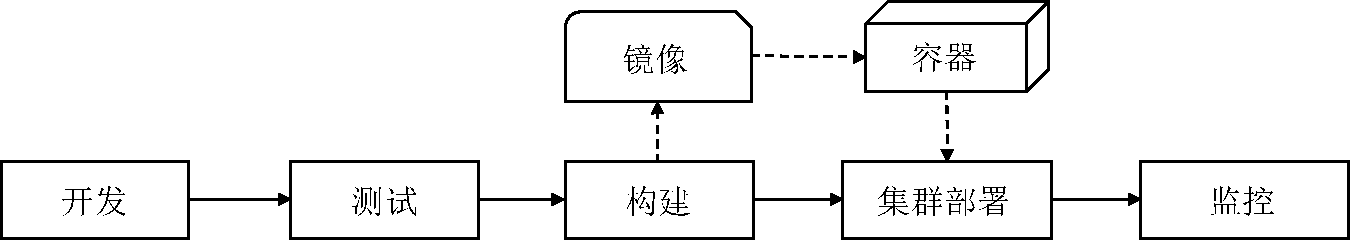
\includegraphics[width=1.0\textwidth]{FIGs/chapter4/deploy_micro_by_container.pdf} %中括号中的参数是设置图片充满文档的大小,你也可以使用小数来缩小图片的尺寸。
    \caption{镜像方式发布微服务流程} %caption是用来给图片加上图题的
    \label{deploy_micro_by_container} %这是添加标签,方便在文章中引用图片。
\end{figure}%figure环境

由于当前智能合约与区块链节点之间是强耦合的关系, 这使得我们很难利用现有工具单独对智能合约进行独立开发、测试、部署、运维。因此, 
本节进行的智能合约微服务化改造流程如图\ref{microservice_for_sc}所示。

\begin{figure}[h] %figure环境,h默认参数是可以浮动,不是固定在当前位置。如果要不浮动,你就可以使用大写float宏包的H参数,固定图片在当前位置,禁止浮动。
    \centering %使图片居中显示
    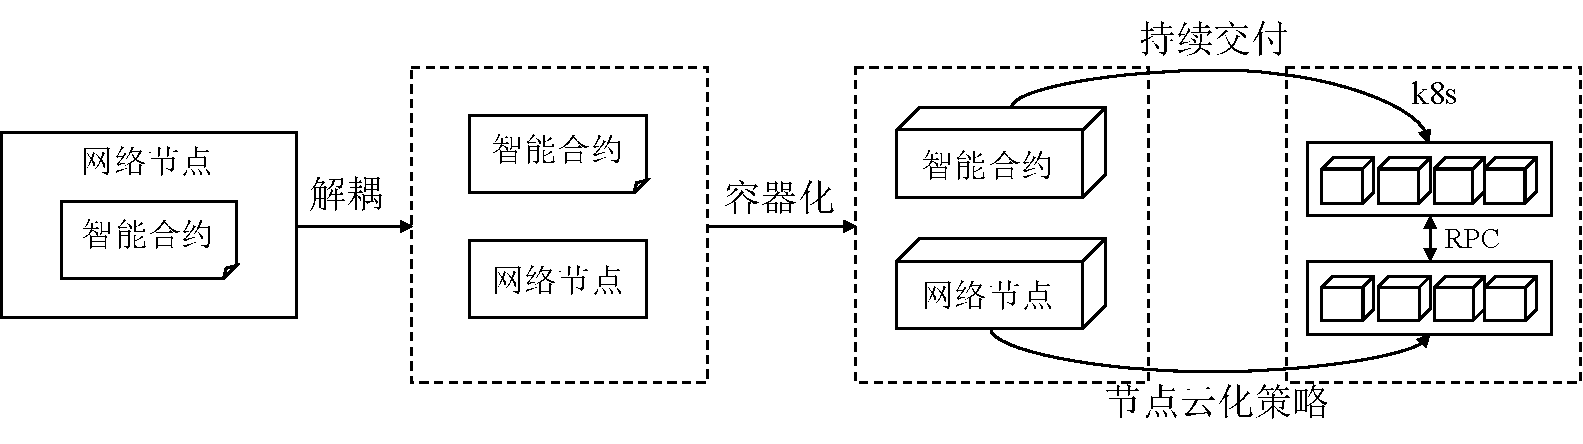
\includegraphics[width=1.0\textwidth]{FIGs/chapter4/microservice_for_sc.pdf} %中括号中的参数是设置图片充满文档的大小,你也可以使用小数来缩小图片的尺寸。
    \caption{智能合约微服务化改造流程} %caption是用来给图片加上图题的
    \label{microservice_for_sc} %这是添加标签,方便在文章中引用图片。
\end{figure}%figure环境

\textbf{(1) 运行环境}

智能合约微服务化改造的目的是解耦, 让智能合约更容易拓展、更富有弹性。在传统的链码安装与实例化的方式中, 链码的构建和运行是HF节点的一部分, 链码和节点之间的耦合度较高, 不具有可复用性。解耦后的智能合约更加专注于自身功能, 不需要关心账本数据的一致性、网络的安全性等问题。解耦后, 需要给智能合约提供容器环境使其可以运行。可以说, 容器化是智能合约与共识节点解耦后平稳运行的基础, 是智能合约微服务化的有效手段。本节将智能合约与网络节点解耦后具备以下优势:

\begin{itemize}[itemindent=2em]
    \item 单一职责: 职责愈加明确, 每个智能合约容器只需要完成自己特定的功能。独立的智能合约能够有效利用现有自动化工具完成持续交付; 

    \item 高融入性\footnotemark[1]\footnotetext[1]{\href{http://pss-system.cnipa.gov.cn/sipopublicsearch/patentsearch/showViewList-jumpToView.shtml}{发明专利: 一种建立智能合约微服务化的方法}}: 智能合约将服务封装成API, 用户可直接将智能合约安插在自己的业务逻辑中;

    \item 高可用性: 利用Kubernetes本身对于高可用性的保障,只需要在Kubernetes层面进行简单的配置(例如Replica、QoS、HPA等),不必针对区块链层面专门进行高可用策略配置;

    \item 高可扩展性: 智能合约进行容器化编排后, 只需要将自己的服务暴露给其他节点及应用。当智能合约需求发生变更时, 只需向集群内部增加新变更的智能合约容器即可。
\end{itemize}


\textbf{(2) 通信机制}

智能合约解耦后需要为智能合约与网络节点提供良好的通信机制, 只有合理有效的通信才能保证智能合约正确的运行。

如表\ref{two_communication}所示, 服务间通信的方式主要有两种, 分别是远程过程调用(Remote Procedure Call, 简称RPC)和表述性状态转移(Representational State Transfer, 简称REST)。这两种方式各有利弊, 存在不同的使用场景。本节的智能合约微服务化改造为保证区块链网络的性能选择RPC的通信方式。

{\footnotesize
\begin{longtable}[h]{m{50pt} m{120pt} m{120pt}}
    \caption[通信机制对比]{通信机制对比} \label{two_communication} \\
        \toprule  
        \textbf{}&\textbf{RPC}&\textbf{REST} \\
        \hline
        场景 & 适用于内部的函数方法调用 & 适用于外部资源接口  \\

        优点 & 性能表现出色 & 便于开发人员理解、调试 \\

        缺点 & 与代码耦合度强, 不方便理解 & 性能表现较差 \\
        \bottomrule
    \end{longtable}
}

\textbf{(3) 持续交付}

持续集成(Continuous Integration, 简称CI)是一种软件开发实践, 团队成员经常集成他们的工作, 通常每个人至少每天都进行集成。每个集成都由自动化的构建(包括测试)进行验证, 以尽可能快地检测集成错误\footnotemark[1]\footnotetext[1]{\href{https://moodle2019-20.ua.es/moodle/pluginfile.php/2228/mod_resource/content/2/martin-fowler-continuous-integration.pdf}{Martin Fowler.Continuous Integration.}}。持续交付(Continuous Delivery, 简称CD)的关注点不在于源码而在于可交付物。

借鉴微服务持续交付的思想, 智能合约从编写完成后就要不断的集成交付。只有持续不断的交付才能持续验证智能合约与下层的区块链云化节点结合的功能完整性。当前, 可交付物从代码制品变为智能合约镜像, 借鉴现有的CI/CD工具(例如Jenkins、Travis CI等)帮助智能合约微服务化开发快速构建持续交付流水线, 可以实现:

\begin{itemize}[itemindent=2em]
    \item 基础设施自动化, 为智能合约微服务化开发降低了构建、部署、交付操作难度,减少集成交付过程中的时间开销;

    \item 频繁的构建升级智能合约, 更早的识别错误, 有效控制风险, 保证代码质量;

    \item 有效的帮助团队成员之间的协作, 促进代码共享, 团队中每个人都能看到构建交付结果。
\end{itemize}


\section{智能合约微服务化开发运维流程}\label{section: smart_contract_micro}

本节智能合约微服务化提供一套从需求、开发、构建、测试、部署到监控的流程指导, 如图\ref{sc_develop}展示了智能合约微服务化开发运维流程以促进智能合约价值交付过程。该图展示的是在已经搭建好的区块链云化网络中, 使用现有自动化工具无侵入的支撑智能合约完整生命周期。

\begin{figure}[h] %figure环境,h默认参数是可以浮动,不是固定在当前位置。如果要不浮动,你就可以使用大写float宏包的H参数,固定图片在当前位置,禁止浮动。
    \centering %使图片居中显示
    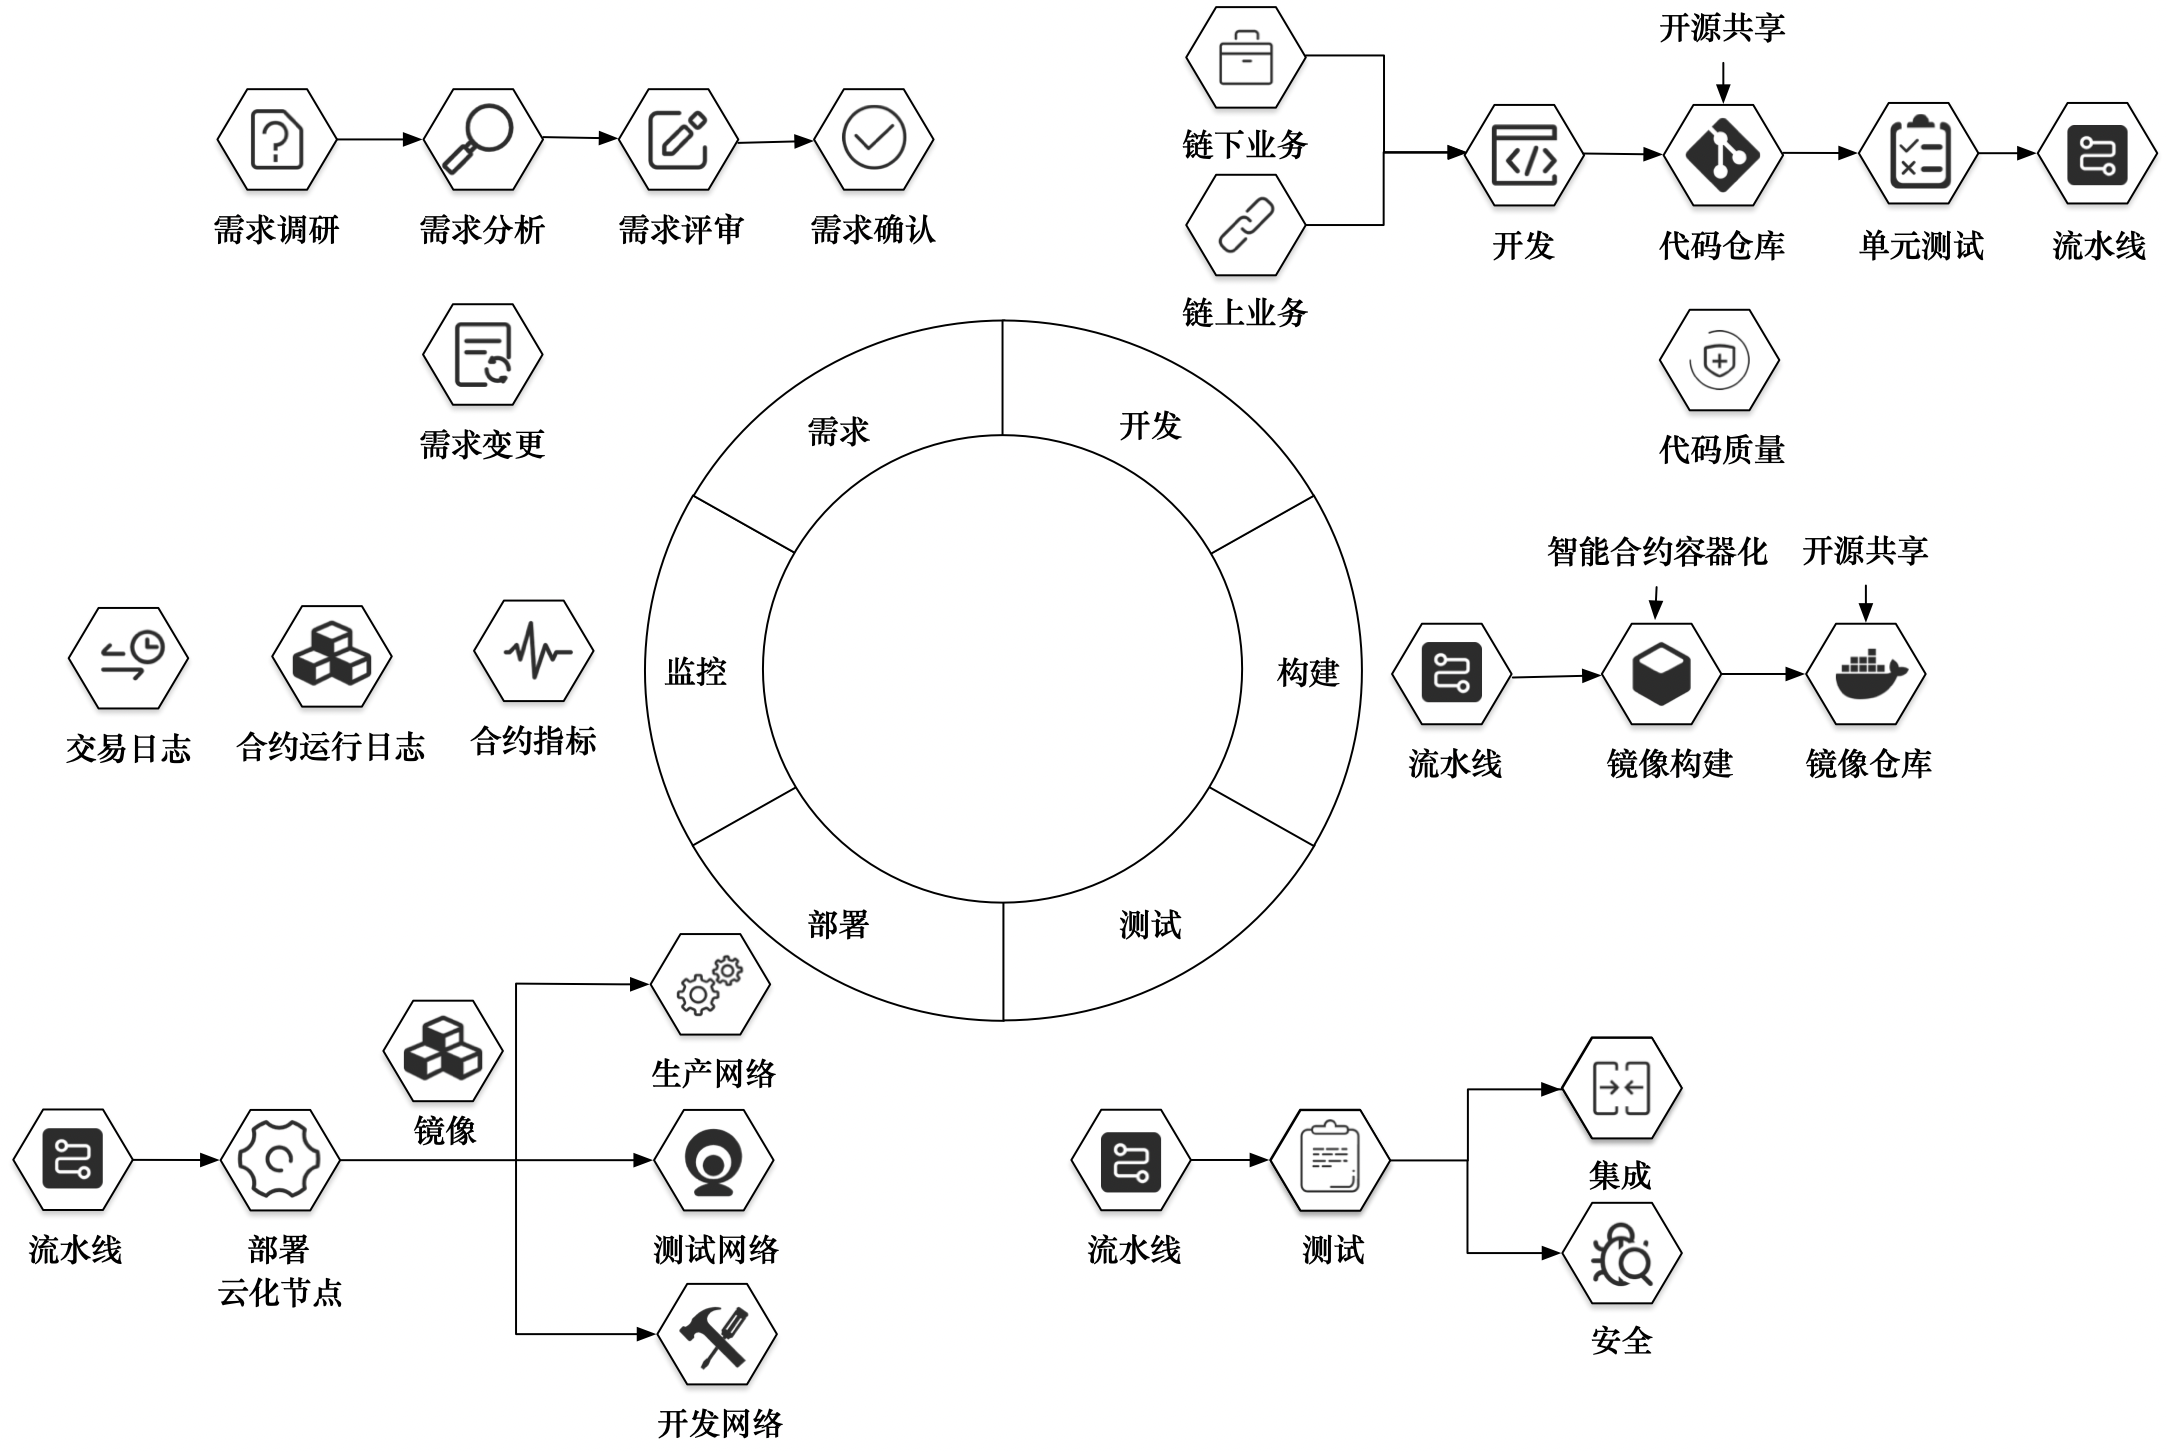
\includegraphics[width=1.0\textwidth]{FIGs/chapter4/process.png} %中括号中的参数是设置图片充满文档的大小,你也可以使用小数来缩小图片的尺寸。
    \caption{智能合约微服务化开发运维流程} %caption是用来给图片加上图题的
    \label{sc_develop} %这是添加标签,方便在文章中引用图片。
\end{figure}%figure环境

\textbf{(1) 需求}

区块链网络是一个典型的分布式网络, 在理论计算机科学中, Eric Brewer提出CAP定理\footnotemark[1]\footnotetext[1]{\href{https://en.wikipedia.org/wiki/CAP_theorem}{CAP Theorem}},分布式数据存储系统中只能同时满足以下三个中的两个:

\begin{itemize}[itemindent=2em]
    \item 一致性(Consistency): 所有节点数据一致性更新;

    \item 可用性(Availability): 系统是否还能在正常时间内响应用户的请求;

    \item 分区可用性(Partition Tolerance): 尽管节点之间的网络丢弃(或延迟)任意数量的消息, 系统仍将继续运行.

\end{itemize}

分布式系统必须满足分区可用性, 即某个节点宕机不会影响其他节点的正常工作, 达到高可靠性。在区块链系统中, 要求所有节点共同维护相同的账本, 所以必须满足一致性原则。在满足上述两个原则的条件下就要牺牲可用性, 系统的响应时间则会变慢。

将一个大的复杂问题,变成多个小问题解决,体现了微服务架构的分而治之的思想。合理的微服务划分是微服务架构成功与否的关键, 但是微服务架构是手段而不是最终的目的。智能合约微服务化改造的最终目的是解耦, 以业务为根本出发点进行抽象划分。为了使去中心化应用具备良好的响应性能,所以在需求分析阶段智能合约需要额外考虑微服务架构在数据处理响应时间方面的区别。区块链的新数据要经过多个节点消耗大量的计算资源才会产生且数据会有多处冗余的备份, 对于大流量数据与实时性要求比较高的数据并不建议使用链上智能合约代码处理, 仅将需要达成共识的数据上链即可。


\textbf{(2) 开发}

当链上业务代码编写完成后托管于代码仓库, 由于现如今智能合约很少开源, 本文提倡以代码库或镜像库的形式分享有用且经过市场检验的智能合约, 促进业界交流, 减少重复开发。开发过程中, 智能合约与其他业务代码隔离, 彼此之间可以使用不同的编程语言。将智能合约开源, 帮助工程师更快了解智能合约内部的工作原理。开发的代码仓库可以对接CI/CD工具, 做到合并代码后自动提交流水线交付。


\textbf{(3) 构建}

智能合约的开发和升级过程都比较繁琐, 所以智能合约的手动部署、版本更迭以及升级过程都容易出错, 这有可能会导致系统漏洞, 甚至升级失败, 造成数据和经济损失。利用已有CI/CD工具实现基础设施自动化,利用容器化工具(如Docker)打包编写完成的智能合约, 衔接测试和部署。同样,将合格的智能合约镜像开源可以方便其他开发者直接部署于自己的区块链网络。

\textbf{(4) 测试}

常见的智能合约漏洞包括重入攻击、事务顺序依赖、时间戳依赖、处理异常、整型溢出等。尽管业界已有各种理论与工具\cite{luu2016making},但自动化程度较低。本文利用持续集成工具提升智能合约测试的自动化水平, 将“可插拔”、“开箱即用”的测试策略配置进入持续交付流水线, 以便在智能合约上链前对其进行全方位测试。

\textbf{(5) 部署}

本文提倡从一开始不断的集成, 将拆分后的智能合约以及区块链共识节点组合起来。每个过程都由自动化的构建(包括测试)进行验证, 以尽可能快地检测集成的错误。智能合约可交付镜像可以在开发、测试、生产环境之间无障碍流通, 打破三者之间的隔阂。开发完成的镜像可以直接交给测试网络测试, 测试完成的镜像可以直接在生产环境中部署。

\textbf{(6) 监控}

在智能合约微服务运行时采用已有监控工具全面采集智能合约容器以及下层区块链云化网络节点的性能指标数据,提供一个标准和定制的性能框架。该框架可以集成数据异常检测、报警、智能决策分析以及可视化。常见的监控指标有:
\begin{itemize}[itemindent=2em]
    \item  响应时间: 每个事务的响应时间,包括平均响应时间、最大响应时间和最小响应时间;

    \item 吞吐量: 每秒成功事务的数量;

    \item 成功率: 成功交易的数量与全部交易数量的比值;

    \item 资源消耗: CPU、内存、磁盘和网络I/O等。

\end{itemize}

\section{原型工具与方法评估}\label{section: smart_contract_microservice_test}

由于本章的智能合约微服务化开发运维方法已经公开发表, 故本节将简要描述基于智能合约微服务化开发运维方法的原型工具Mictract核心工作原理以及智能合约微服务化开发运维方法的评估过程。

如图\ref{mictract}所示, Mictract\footnotemark[1]\footnotetext[1]{\href{https://github.com/doporg/Mictract}{Java for Mictract}}\footnotemark[2]\footnotetext[2]{\href{https://github.com/doporg/Mictract-go-server}{Go for Mictract}}作为传统BaaS平台能够为构建区块链应用程序的人或组织提供第三方区块链服务, 允许用户构建、托管、运行、监控自己的区块链应用。Mictract的核心优势是具备BaaS平台基本功能的前提下, 屏蔽了底层方法原理与工具, 形成了支撑智能合约开发运维的工具链。值得注意的是, Mictract搭建的下层区块链网络与传统BaaS平台类似, 只是简单的将区块链网络迁移上云。因此, Mictract在下层网络节点云化方面存在一定的不足, 需要整合区块链节点云化方案形成完整的区块链云化框架。

\begin{figure}[h] %figure环境,h默认参数是可以浮动,不是固定在当前位置。如果要不浮动,你就可以使用大写float宏包的H参数,固定图片在当前位置,禁止浮动。
    \centering %使图片居中显示
    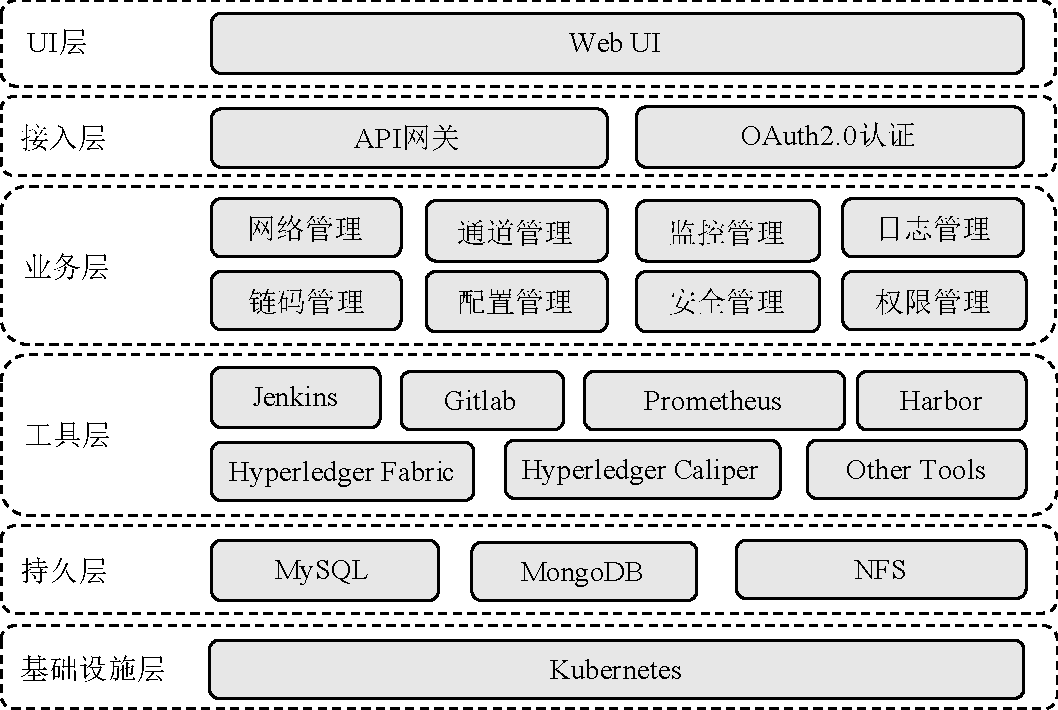
\includegraphics[width=0.9\textwidth]{FIGs/chapter4/mictract.pdf} %中括号中的参数是设置图片充满文档的大小,你也可以使用小数来缩小图片的尺寸。
    \caption{Mictract架构图} %caption是用来给图片加上图题的
    \label{mictract} %这是添加标签,方便在文章中引用图片。
\end{figure}%figure环境

将官方HF的链码打包成Docker镜像并将这些镜像部署于Kubernetes是智能合约微服务化的基础也是阻碍智能合约微服务化的主要问题。HF 2.0引入了链码新生命周期, 工程师通过新生命周期命令可以打包新类型链码包, 并生成一个链码包的packageID。原型工具利用伪代码\ref{cc_dockerfile}将链码打包成Docker镜像。当需要部署链码时, 利用伪代码\ref{code4}配置链码的部署文件,拉取链码镜像并为其配置环境变量, 最终生成相应的Kubernetes Pod容器作为独立的运行单元。除了对上述镜像及Deployment的改造外, Mictract在核心部署环节还存在三个难点:

\begin{itemize}[itemindent=2em]
    \item  Kubernetes部署Deployment时, Kubernetes在非人为指定下会选择出集群中适合运行当前Pod资源的一个节点, 这种资源调度策略很可能使Pod与证书文件、初始区块或者通道文件处于不同节点, 所以采用NFS文件服务器的方式将上述配置文件共享;

    \item Mictract将packageID等环境变量和共享的配置文件以Deployment容器变量的形式传入;

    \item 将Peer声明为外部链码构建形式并为其传入外部链码构建器启动器。同时, 将Peer节点生成外部链码标识符传入外部链码的Deployment容器。
\end{itemize}

\begin{algorithm}[!htbp]
    \floatname{algorithm}{\footnotesize 伪代码}
    \caption{\footnotesize 智能合约Dockerfile伪代码}
    \label{cc_dockerfile}
    {\footnotesize
    \begin{algorithmic}
        \renewcommand{\algorithmicrequire}{ \textbf{Input:}}
        \REQUIRE  
        智能合约代码
        \renewcommand{\algorithmicensure}{\textbf{Output:}}
        \ENSURE
        暴露端口提供服务

        \STATE{FROM <base-image:tage>}
        \STATE{COPY <src> <dest>}
        \STATE{WORKDIR <dest> }
        \STATE{RUN <build-command>}
        \STATE{EXPOSE <port>}
        \STATE{CMD <run-command>}
    \end{algorithmic}
    }
\end{algorithm}

\begin{algorithm}[!htbp]
    \floatname{algorithm}{\footnotesize 伪代码}
    \caption{\footnotesize 智能合约 Deployment伪代码}
    \label{code4}
    {\footnotesize
    \begin{algorithmic}
        \renewcommand{\algorithmicrequire}{ \textbf{Input:}}
        \REQUIRE  
        链码镜像地址, 命名空间, 链码包packageID
        \renewcommand{\algorithmicensure}{\textbf{Output:}}
        \ENSURE
        暴露端口提供服务

        \STATE{namespace <namespace>}
        \STATE{containers: image <image-uri>}
        \STATE{image: imagePullPolicy <IFNotPresent>}
        \STATE{env: CHAINCODE-PACKAGEID <packageID>}
        \STATE{env: CHAINCODE-ADDRESS <address>}
        \STATE{container: port <port>}
    \end{algorithmic}
    }
\end{algorithm}

在测试方面, Mictract提供对Go语言编写链码的测试, 其借鉴HF的 MockStub类完成账本初始化工作, 采用MockStub类单元测试以及性能测试, 利用pprof\footnotemark[1]\footnotetext[1]{\href{https://github.com/google/pprof}{go pprof github地址}}完成性能剖析工作; 在智能合约监控层面, Mictract提供智能合约资源消耗以及交易过程监控两个方面的监控。

为了验证本节提出的智能合约微服务化开发运维方法的可行性与部署效率, 本节选取了官方链码asset进行案例研究, 使用智能合约微服务化开发运维方法对asset进行托管、运行、监控。可行性是本文首要关心的问题, 智能合约微服务化开发运维方法需保证智能合约运行无误。为此本文将官方asset链码进行微服务化改造, 验证其是否满足预期功能。操作过程如下表\ref{operator_chaincode}所示, 该表为表明智能合约微服务化开发运维方法确保智能合约正确运行, 并不是为了展示asset链码本身的功能, 故未进行全部功能的调用。结果表明, 智能合约微服务化改造满足预期, 可以保证智能合约运行的正确。

目前, 缺乏智能合约微服务化的有效评估指标。由于智能合约微服务化开发运维方法的目的是利用已有的成熟工具快速部署、操作、监控智能合约, 以此来提升智能合约开发运维自动化水平, 故本文选取部署效率作为分析指标。表\ref{experimental_results_of_smart contract_micro_service}展示了采用官方脚本方式以及智能合约微服务化开发运维方法搭建、部署不同网络规模所消耗的时间。由于Peer节点的数量、组织的数量以及通信效率的影响, 同一规格的网络部署时间可能会略有差别。在环境完备且中间不出现Bug的前提下采用脚本方式比智能合约微服务化开发运维方法平均多使用225.6秒。该方法整合进入面向Hyperledger Fabric的区块链云化框架后与官方BaaS平台Cello针对链码部署效率的对比情况详见第\ref{section: tool_comparison}节。

{\footnotesize
\begin{longtable}[h]{l m{90pt} m{210pt} l}
    \caption[操作链码实例]{操作链码实例} \label{operator_chaincode}\\
        \toprule  
        \textbf{步骤}&\textbf{操作}&\textbf{预期结果}&\textbf{实际}\\
        \hline
        step1 & InitLedger() & txid=<TXID> & 通过 \\
        \hline
        step2 & GetAllAssets() & [\{“Key”:“asset1”,“Record”:\{“ID”:“asset1”,“color”:“blue”,“size”:5,“owner”:“Tomoko”,“appraisedValue”:300\}\}, 
        \newline \{“Key”:“asset2”,“Record”:\{“ID”:“asset2”,“color”:“red”, “size”:5,“owner”:“Brad”,“appraisedValue”:400\}\}] & 通过 \\
        \hline
        step3 & ReadAsset(“asset1”) & \{“ID”:“asset1”,“color”:“blue”,“size”:5,“owner”:“Tomoko”,
        "appraisedValue":300\} txid=<TXID> & 通过 \\
        \hline
        step4 & TransferAsset(“asset1”, “Brad”) & Tomoko txid=<TXID>   & 通过 \\
        \hline
        step5 & ReadAsset(“asset1”) & \{“ID”:“asset1”,“color”:“blue”,“size”:5,“owner”:“Brad”,
        "appraisedValue":300\} txid=<TXID>  & 通过 \\
        \bottomrule
        
    \end{longtable} 
}

{\footnotesize
\begin{longtable}[h]{ccccc}
    \caption[部署效率对比(单位: 秒(s))]{部署效率对比(单位: 秒(s))} \label{experimental_results_of_smart contract_micro_service}\\
        \toprule  
        \textbf{总Peer数}&\textbf{总Orderer数}&\textbf{组织数量}&\textbf{脚本方式}&\textbf{智能合约微服务化方法}\\
        \hline
        2 & 2 & 2 & 342 & 136\\
        4 & 3 & 2 & 440 & 185\\
        2 & 3 & 2 & 358 & 146\\
        3 & 4 & 3 & 483 & 202\\
        1 & 2 & 1 & 306 & 132\\
        \bottomrule
    \end{longtable} 
}

\section{本章小结}

本章首先分析了智能合约开发运维过程中的挑战, 并分析了智能合约与微服务架构在设计原则上的相似性, 结果表明智能合约与微服务都具备相似的特性。基于这种相似性, 本章随后阐述了智能合约微服务化改造过程, 包含核心的解耦思想、运行环境以及通信机制, 然后提出了智能合约微服务化开发运维流程。最后, 本章介绍了方法的原型工具并对所提方法进行了可行性与部署效率的评估。